% respuesta2.tex

Al correr el programa, que calcula el resultado del método de Newton para resolver la equacion

\begin{equation*}
	\frac{1}{4} x^{2} - x \sin{x} - \frac{1}{2} \cos{2x} + \frac{1}{2} = 0
\end{equation*}
con los siguientes puntos iniciales 
\begin{equation*}
	[\frac{\pi}{2}, 5\pi, 10\pi]
\end{equation*}
obtenemos la siguiente información: 


\begin{figure}[H]
	\centering
	\caption{Punto inicial: $\pi$ \converge}
	\begin{tabular}{|c|c|c|c|} \hline
		$i$ & $x_{i}$ & $f(x_{i})$ & $f'(x_{i})$ \\ \hline
		$0$ & $1.7853982$ & $0.0460539$ & $-0.2146018$ \\ \hline
		$1$ & $1.8445616$ & $0.0071170$ & $-0.1202935$ \\ \hline
		$2$ & $1.8708344$ & $0.0016385$ & $-0.0623666$ \\ \hline
		$3$ & $1.8833464$ & $0.0003963$ & $-0.0316759$ \\ \hline
		$4$ & $1.8894638$ & $0.0000976$ & $-0.0159548$ \\ \hline
		$5$ & $1.8924896$ & $0.0000242$ & $-0.0080059$ \\ \hline
		$6$ & $1.8939946$ & $0.0000060$ & $-0.0040100$ \\ \hline
		$7$ & $1.8947451$ & $0.0000015$ & $-0.0020068$ \\ \hline
		$8$ & $1.8951198$ & $0.0000004$ & $-0.0010038$ \\ \hline
		$9$ & $1.8953071$ & $0.0000001$ & $-0.0005020$ \\ \hline
		$10$ & $1.8954007$ & $0.0000000$ & $-0.0002510$ \\ \hline
		$11$ & $1.8954475$ & $0.0000000$ & $-0.0001255$ \\ \hline
		$12$ & $1.8954709$ & $0.0000000$ & $-0.0000628$ \\ \hline
		$13$ & $1.8954826$ & $0.0000000$ & $-0.0000314$ \\ \hline
		$14$ & $1.8954884$ & $0.0000000$ & $-0.0000157$ \\ \hline
		$15$ & $1.8954913$ & $0.0000000$ & $-0.0000078$ \\ \hline
		$16$ & $1.8954928$ & $0.0000000$ & $-0.0000039$ \\ \hline
		$17$ & $1.8954935$ & $0.0000000$ & $-0.0000020$ \\ \hline
		$18$ & $1.8954939$ & $0.0000000$ & $-0.0000010$ \\ \hline
		$19$ & $1.8954941$ & $0.0000000$ & $-0.0000005$ \\ \hline
		$20$ & $1.8954942$ & $0.0000000$ & $-0.0000002$ \\ \hline
		$21$ & $1.8954942$ & $0.0000000$ & $-0.0000001$ \\ \hline
		$22$ & $1.8954942$ & $0.0000000$ & $-0.0000001$ \\ \hline
	\end{tabular}
\end{figure}

\begin{figure}[H]
	\centering
	\caption{Punto inicial: $5\pi$ \converge}
	\begin{tabular}{|c|c|c|c|} \hline
		$i$ & $x_{i}$ & $f(x_{i})$ & $f'(x_{i})$ \\ \hline
		$0$ & $13.0899694$ & $61.6850275$ & $23.5619449$ \\ \hline
		$1$ & $21.3475720$ & $36.5418400$ & $-4.4252359$ \\ \hline
		$2$ & $17.4729273$ & $101.4799493$ & $26.1907751$ \\ \hline
		$3$ & $1.6486799$ & $94.4331539$ & $5.9676237$ \\ \hline
		$4$ & $1.7980631$ & $0.0298006$ & $-0.1994913$ \\ \hline
		$5$ & $1.8499401$ & $0.0056632$ & $-0.1091663$ \\ \hline
		$6$ & $1.8733573$ & $0.0013193$ & $-0.0563373$ \\ \hline
		$7$ & $1.8845720$ & $0.0003203$ & $-0.0285638$ \\ \hline
		$8$ & $1.8900682$ & $0.0000790$ & $-0.0143762$ \\ \hline
		$9$ & $1.8927898$ & $0.0000196$ & $-0.0072112$ \\ \hline
		$10$ & $1.8941442$ & $0.0000049$ & $-0.0036113$ \\ \hline
		$11$ & $1.8948197$ & $0.0000012$ & $-0.0018071$ \\ \hline
		$12$ & $1.8951571$ & $0.0000003$ & $-0.0009039$ \\ \hline
		$13$ & $1.8953257$ & $0.0000001$ & $-0.0004520$ \\ \hline
		$14$ & $1.8954100$ & $0.0000000$ & $-0.0002260$ \\ \hline
		$15$ & $1.8954521$ & $0.0000000$ & $-0.0001130$ \\ \hline
		$16$ & $1.8954732$ & $0.0000000$ & $-0.0000565$ \\ \hline
		$17$ & $1.8954837$ & $0.0000000$ & $-0.0000283$ \\ \hline
		$18$ & $1.8954890$ & $0.0000000$ & $-0.0000141$ \\ \hline
		$19$ & $1.8954916$ & $0.0000000$ & $-0.0000071$ \\ \hline
		$20$ & $1.8954930$ & $0.0000000$ & $-0.0000035$ \\ \hline
		$21$ & $1.8954936$ & $0.0000000$ & $-0.0000018$ \\ \hline
		$22$ & $1.8954939$ & $0.0000000$ & $-0.0000009$ \\ \hline
		$23$ & $1.8954941$ & $0.0000000$ & $-0.0000004$ \\ \hline
		$24$ & $1.8954942$ & $0.0000000$ & $-0.0000002$ \\ \hline
		$25$ & $1.8954942$ & $0.0000000$ & $-0.0000001$ \\ \hline
		$26$ & $1.8954942$ & $0.0000000$ & $-0.0000001$ \\ \hline
		$27$ & $1.8954943$ & $0.0000000$ & $-0.0000000$ \\ \hline
	\end{tabular}
\end{figure}


\begin{center}
	\captionof{figure}{Punto inicial: $10\pi$ \converge}
	\begin{longtable}{|c|c|c|c|} \hline
		$i$ & $x_{i}$ & $f(x_{i})$ & $f'(x_{i})$ \\ \hline
		$0$ & $47.1238898$ & $246.7401100$ & $-15.7079633$ \\ \hline
		$1$ & $39.2699082$ & $555.1652476$ & $70.6858347$ \\ \hline
		$2$ & $20.6349541$ & $347.2615137$ & $18.6349541$ \\ \hline
		$3$ & $14.0844908$ & $87.2433669$ & $13.3186561$ \\ \hline
		$4$ & $7.3295384$ & $36.5254936$ & $5.4072170$ \\ \hline
		$5$ & $1921.5404903$ & $7.8353322$ & $-0.0040932$ \\ \hline
		$6$ & $-6212.1139178$ & $924804.9759238$ & $113.7010413$ \\ \hline
		$7$ & $-4438.8695742$ & $9653346.7729376$ & $-5443.8897877$ \\ \hline
		$8$ & $-3689.0763974$ & $4925005.2698354$ & $-6568.4850462$ \\ \hline
		$9$ & $-9361.6753668$ & $3399558.4368288$ & $599.2946893$ \\ \hline
		$10$ & $-14410.6158688$ & $21912745.2270146$ & $4340.0680238$ \\ \hline
		$11$ & $-11995.1385095$ & $51918335.7955691$ & $-21494.0270898$ \\ \hline
		$12$ & $-20350.8637606$ & $35964693.1763045$ & $4304.1976723$ \\ \hline
		$13$ & $-32153.6935851$ & $103546838.6734365$ & $8773.0519048$ \\ \hline
		$14$ & $-26303.8986398$ & $258449384.2733945$ & $-44180.9305611$ \\ \hline
		$15$ & $-21214.5387407$ & $172957713.6523489$ & $-33984.1781835$ \\ \hline
		$16$ & $-17148.2210877$ & $112501555.1255755$ & $-27666.6912741$ \\ \hline
		$17$ & $-4477.3764256$ & $73498450.0392219$ & $-5800.5959349$ \\ \hline
		$18$ & $-3630.0860097$ & $5014278.7724454$ & $-5918.0166310$ \\ \hline
		$19$ & $-1898.2094594$ & $3298011.1230452$ & $-1904.2991964$ \\ \hline
		$20$ & $-3636.3713853$ & $899595.5784556$ & $517.5556805$ \\ \hline
		$21$ & $-1894.2216866$ & $3309435.6950319$ & $-1899.6276252$ \\ \hline
		$22$ & $-1575.9045549$ & $896719.6524757$ & $-2817.0637499$ \\ \hline
		$23$ & $1871.4510788$ & $622323.6879867$ & $-180.5220447$ \\ \hline
		$24$ & $7001.0593921$ & $877092.1883610$ & $-170.9861913$ \\ \hline
		$25$ & $3637.1758662$ & $12246709.5161439$ & $3640.6461228$ \\ \hline
		$26$ & $8075.3076376$ & $3309842.2222794$ & $-745.7737608$ \\ \hline
		$27$ & $2214.1410621$ & $16294672.4394335$ & $2780.1073779$ \\ \hline
		$28$ & $1780.7410806$ & $1224210.2955517$ & $2824.6662390$ \\ \hline
		$29$ & $1452.7934396$ & $791841.4393738$ & $2414.5361647$ \\ \hline
		$30$ & $275.3098815$ & $526227.3832642$ & $446.9084767$ \\ \hline
		$31$ & $-479.7389156$ & $19201.0395684$ & $25.4301969$ \\ \hline
		$32$ & $-371.2700565$ & $57154.9340550$ & $-526.9248201$ \\ \hline
		$33$ & $-638.6617194$ & $34262.7667743$ & $128.1370047$ \\ \hline
		$34$ & $-494.0812020$ & $102480.3341694$ & $-708.8115050$ \\ \hline
		$35$ & $-387.1924527$ & $61401.1941242$ & $-574.4401962$ \\ \hline
		$36$ & $-307.1248467$ & $37751.3449524$ & $-471.4933647$ \\ \hline
		$37$ & $-641.2088390$ & $23791.5089290$ & $71.2141541$ \\ \hline
		$38$ & $-998.6794801$ & $102583.1971350$ & $286.9695727$ \\ \hline
		$39$ & $-1565.9782382$ & $249679.9054533$ & $440.1206628$ \\ \hline
		$40$ & $-574.8496464$ & $611515.7109923$ & $-616.9892747$ \\ \hline
		$41$ & $-478.9398636$ & $82577.5244163$ & $-860.9916736$ \\ \hline
		$42$ & $-135.8801421$ & $56873.4811346$ & $-165.7830330$ \\ \hline
		$43$ & $-107.3387362$ & $4713.0408533$ & $-165.1299474$ \\ \hline
		$44$ & $-180.0664384$ & $2826.8908166$ & $38.8695192$ \\ \hline
		$45$ & $-136.5431877$ & $8257.7814073$ & $-189.7326436$ \\ \hline
		$46$ & $-80.3063845$ & $4797.6211971$ & $-85.3110584$ \\ \hline
		$47$ & $-12.9785910$ & $1692.0133666$ & $-25.1309790$ \\ \hline
		$48$ & $-20.2925756$ & $37.0716685$ & $5.0686009$ \\ \hline
		$49$ & $-8.0070693$ & $83.8037739$ & $-6.8213529$ \\ \hline
		$50$ & $-5.6965144$ & $9.0916100$ & $-3.9348167$ \\ \hline
		$51$ & $-10.8076459$ & $11.5725758$ & $2.2641905$ \\ \hline
		$52$ & $-6.1585544$ & $40.7837593$ & $-8.7724148$ \\ \hline
		$53$ & $-9.4126197$ & $10.2629614$ & $3.1538892$ \\ \hline
		$54$ & $-7.8478253$ & $22.0350615$ & $-14.0817616$ \\ \hline
		$55$ & $-4.8874436$ & $8.5493760$ & $-2.8879303$ \\ \hline
		$56$ & $0.3735117$ & $11.7541929$ & $-2.2342316$ \\ \hline
		$57$ & $0.1668875$ & $0.0317308$ & $0.1535677$ \\ \hline
		$58$ & $0.0818546$ & $0.0068344$ & $0.0803730$ \\ \hline
		$59$ & $0.0407434$ & $0.0016676$ & $0.0405625$ \\ \hline
		$60$ & $0.0203491$ & $0.0004145$ & $0.0203266$ \\ \hline
		$61$ & $0.0101717$ & $0.0001035$ & $0.0101689$ \\ \hline
		$62$ & $0.0050855$ & $0.0000259$ & $0.0050852$ \\ \hline
		$63$ & $0.0025427$ & $0.0000065$ & $0.0025427$ \\ \hline
		$64$ & $0.0012714$ & $0.0000016$ & $0.0012713$ \\ \hline
		$65$ & $0.0006357$ & $0.0000004$ & $0.0006357$ \\ \hline
		$66$ & $0.0003178$ & $0.0000001$ & $0.0003178$ \\ \hline
		$67$ & $0.0001589$ & $0.0000000$ & $0.0001589$ \\ \hline
		$68$ & $0.0000795$ & $0.0000000$ & $0.0000795$ \\ \hline
		$69$ & $0.0000397$ & $0.0000000$ & $0.0000397$ \\ \hline
		$70$ & $0.0000199$ & $0.0000000$ & $0.0000199$ \\ \hline
		$71$ & $0.0000099$ & $0.0000000$ & $0.0000099$ \\ \hline
		$72$ & $0.0000050$ & $0.0000000$ & $0.0000050$ \\ \hline
		$73$ & $0.0000025$ & $0.0000000$ & $0.0000025$ \\ \hline
		$74$ & $0.0000012$ & $0.0000000$ & $0.0000012$ \\ \hline
		$75$ & $0.0000006$ & $0.0000000$ & $0.0000006$ \\ \hline
		$76$ & $0.0000003$ & $0.0000000$ & $0.0000003$ \\ \hline
		$77$ & $0.0000002$ & $0.0000000$ & $0.0000002$ \\ \hline
		$78$ & $0.0000001$ & $0.0000000$ & $0.0000001$ \\ \hline
		$79$ & $0.0000000$ & $0.0000000$ & $0.0000000$ \\ \hline
		$80$ & $0.0000000$ & $0.0000000$ & $0.0000000$ \\ \hline
	\end{longtable}
\end{center}


\begin{figure}[H]
	\centering
	\begin{minipage}{0.45\textwidth}
		\caption{Desde -30 a 30}		
		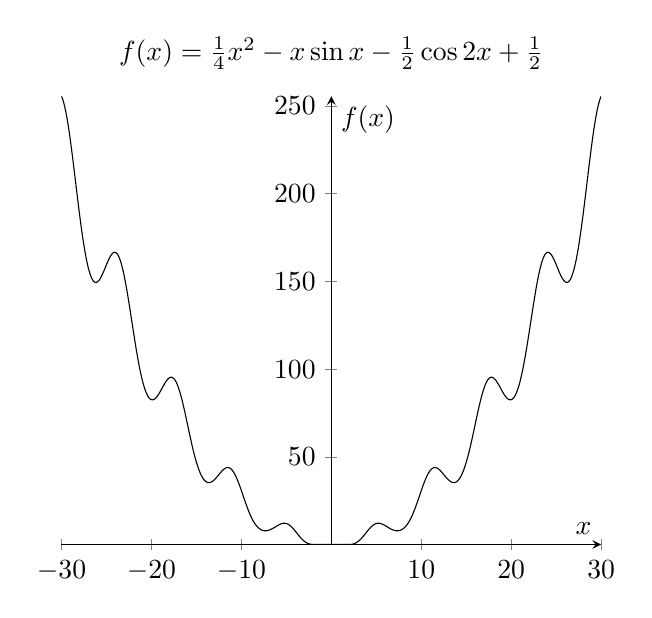
\begin{tikzpicture}
		\begin{axis}[ 
		title={$f(x) = \frac{1}{4} x^{2} - x \sin{x} - \frac{1}{2} \cos{2x} + \frac{1}{2}$},
		xlabel=$x$,
		ylabel=$f(x)$,
		axis lines=center,
		% axis on top=true,
		] 
		\addplot [domain=-30:30,samples=500]{0.25 * (x*x) - x * sin(deg(x)) - 0.5 * cos(deg(2*x)) + 0.5};
		\end{axis}
		\end{tikzpicture}
	\end{minipage}\hfill
	\begin{minipage}{0.45\textwidth}
		\caption{Desde -3 a 3}
		\begin{tikzpicture}
		\begin{axis}[ 
		title={$f(x) = \frac{1}{4} x^{2} - x \sin{x} - \frac{1}{2} \cos{2x} + \frac{1}{2}$},
		xlabel=$x$,
		ylabel=$f(x)$,
		axis lines=center,
		% axis on top=true,
		] 
		\addplot [domain=-3:3,samples=500]{0.25 * (x*x) - x * sin(deg(x)) - 0.5 * cos(deg(2*x)) + 0.5}; 
		\end{axis}
		\end{tikzpicture}
	\end{minipage}
\end{figure}

El método converge en los 3 casos aunque no con la velocidad que esperaríamos de este método. \\
En el primer ($x_{0} = \pi/2$) caso se debe a la cercanía que tiene la curva con el eje x, por lo que al trazar
las rectas tangentes, no hay mucho avance. \\
En los otros dos casos de ($x_{0} = 5\pi$ y $x_{0} = 10\pi$) se debe a las irregularidades de la curva,
en $x_{0} = 5\pi$ se pierde pero no tarda tanto en converger, y luego tarda por las mismas, ya que en este punto no existen tantas regularidades
entre la solución y el punto inicial.
Con $x_{0} = 10\pi$, tarde en coverger por la pendiente al trazar las rectas tangentes toma un punto pero como la 
pendiente cambia su sentido de manera irregular entonces el método se pierde y por eso tarda en encontrar la solución.

